\documentclass[a4paper]{article}
\usepackage[utf8]{inputenc}
\usepackage{graphicx}
\graphicspath{ {./images/} }
\usepackage{hyperref}
\hypersetup{
    colorlinks=true,
    urlcolor=blue,
    citecolor=black,
    }
\urlstyle{same}
\usepackage[fontsize=9pt]{fontsize}
\begin{document}

\title{COMP3100 project report}
\hrule \medskip
\begin{minipage}{0.9\textwidth}
\centering 
\large
Stage 2 COMP3100 Distributed Systems, S2, 2022\\
\normalsize
SID: 45334625, Name: Shakeel Mohammed
\end{minipage}
\medskip\hrule
\bigskip

\section{Introduction}
What is this project?
This report presented is to describe the overview, design, implementation, and evaluation of an optimised scheduling system over the previous algorithm described in it's stage 1 counterpart \cite{s1-report}. 

The goal of the optimisation is the reduce the average turn around time of jobs scheduled compared to the 4 baseline scheduling algorithms; First-Capable, First-Fit, Best-Fit, and Worst-Fit. The results generated by the first script found in this project will highlight the benefits and drawback of the optimised algorithm when compared to each of the 4 baseline algorithms.

At it's core, a distributed system is a system that has various components which are spread across a network. This provides many advantages such as efficiency and redundancy, it also introduces complications such as an increased complexity, synchronisation and replication issues.

In a distributed system, the load is distributed across multiple machines to achieve fast and more reliable results. Each distributed system requires a component to orchestrate and distribute each request.

This project acts as an orchestrating component of a distributed system.

The goal for this project is to have a client which connects to the server, and makes scheduling decisions that result in an optimised turnaround time in the processing of each job when compared to the 4 baseline algorithms.

\section{Problem Definition}
\label{sec:section2}
First-Capable, First-Fit, Best-Fit, and Worst-Fit (baseline algorithms) all work differently, each providing advantages and disadvantages for certain workloads:
\begin{enumerate}
  \item First-Capable - allocates jobs to the first machine capable of handing the job, ignoring the number of jobs already in queue for that machine. This proves to be efficient in terms of cost, but inefficient in terms of turnaround times due to the increased queue times.
  \item First-Fit - allocates jobs to the first machine that is capable of handling the job immediately, this proves to be efficient in terms of turnaround time, but can lead to poor resource utilisation as it can leave unused cores on each machine. 
  \item Best-Fit - allocates the job to a machine which is the least sufficient among the available machines, but may perform poorer than other algorithms in some cases as it can leave cores that can't be used since jobs cannot be broken up and handled separately.
  \item Worst-Fit - allocates the job to a machine which is the most sufficient among the available machines, resulting in more compute resources left on the machine in anticipation for the next job, but it leads to an increased cost and poor utilisation if the remaining jobs require more than the leftover resources on the machine.
\end{enumerate}

The objective of this project is design an algorithm that reduces average turnaround time when compared to each of these baseline algorithms without sacrificing too much of the other performance metrics such as resource utilisation and server rental cost.

\section{Algorithm Description}
\label{sec:section3}
The algorithm designed as part of this project is able to produce shorter turnaround times for job scheduling than all 4 of the baseline algorithms in certain circumstances by combining the methods used by the First-Capable and Best-Fit algorithms.

This is demonstrated most effectively in scheduling configurations where there are N servers currently processing jobs at full capacity before another job comes in. The job is scheduled to the least capable server that can handle the job once it becomes available.

When a new job comes in, the algorithm performs a GETS CAPABLE command based on the job and sorts the response by estimated job wait time per server in ascending order. The algorithm then loops over the sorted list, searching for the first server that can handle the job immediately and schedules the job with that server if found. If there is no server that can handle the job immediately, the job is queued for the server that is least sufficient in handling the job in terms of core count.

\begin{center}
    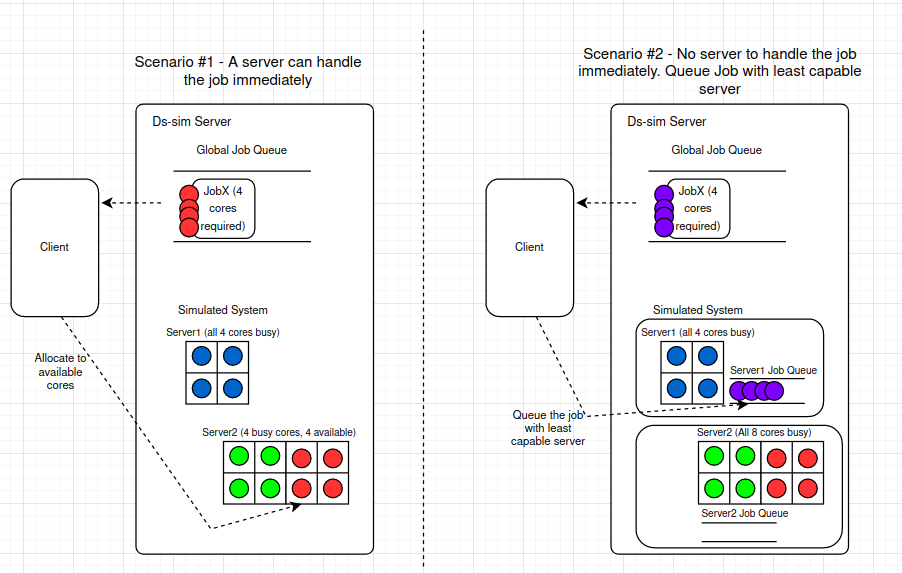
\includegraphics[scale=0.3]{images/job-scheduling.png}
\end{center}

This can be most easily observed in the \verb|config20-short-high.xml| configuration file found in the \verb|/testing/aarch64/S2DemoConfigs| directory.

The average turnaround-time produced by this algorithm could be further optimised by performing a calculation before moving to least capable server to see when the next preferred server will become free and either still schedule the job or migrate the currently running job is it recently started.

\section{Implementation}
\label{sec:section4}
Java 1.8 - Java is a programming language and computing platform first released by Sun Microsystems in 1995. It has evolved from humble beginnings to power a large share of today’s digital world \cite{java}.

As highlighted in the stage 1 counterpart for this report, this project still makes use of the core components such as the ConfigDataLoader, ClientServerConnection, Orchestrator, SimulatedSystem, SimulatedServer and Job classes to handle the client-server connection, data processing and manipulation, and fundamental scheduling functionality. 

The biggest change introduced in stage 2 is the adoption of using the Java Collections and Comparator libraries to help manage the sorting of ArrayLists. In addition to the libraries highlighted in the stage 1 counterpart for this report, this project employs the use of the following classes provided by Java 1.8:
\begin{enumerate}
  \item Sorted Arraylists - Utilising the Java Collections and Comparator libraries to sort SimulatedServers based on key metrics such as core count, estimated job wait time, etc.
  \item Collections - The SimulatedSystem employs the use of the Java Collections library to sort lists of SimulatedServers.
  \item Comparator - The SimulatedSystem employs the use of the Java Comparator library to compare SimulatedServers whilst performing sorting operations.
\end{enumerate}

\section{Evaluation}
\label{sec:section5}
\subsection{Compile}
A pre-compiled version of this project can be found in the \verb|/compiled| directory. Otherwise, run \verb|bash compile.bash| from the \verb|/scripts| directory to compile the files in the \verb|/src| directory and overwrite the files in the \verb|/compiled| directory.

\subsection{Simulation Setup}
A simulation can be run by running the \verb|{cpu_architecture}_test.bash| script from the \verb|/scripts| directory. For aarch64 architecture, run \verb|aarch64_test.bash|. For x86 architecture, run \verb|x86_test.bash|.

Running the appropriate script for the architecture of the machine used will run the algorithm against all of the test configurations. Once complete, a comparison of the results between the newly designed algorithm and the 4 baseline algorithms when run with each configuration will be displayed as such:

\begin{center}
    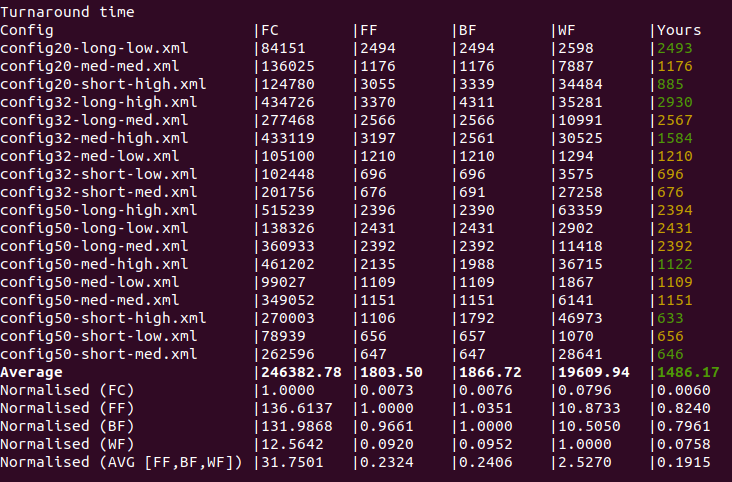
\includegraphics[scale=0.35]{images/simulation-result.png}
\end{center}

Results are highlighted the following colors:
\begin{itemize}
  \item Green - If the result is more efficient than all 4 of the baseline algorithms.
  \item Orange - If the result is more efficient than at least one of the 4 baseline algorithms.
  \item Red - If the result is less efficient than the least efficient of the baseline algorithms.
\end{itemize}

Additionally, we can observe an average of how each of the algorithms performed for each metric across all configurations.

\subsection{Observations}
By running the tests, we can observe that the average turnaround time is greatly reduced in comparison to the 4 baseline algorithms, with fastest algorithm on average being first-fit at an average of 1803.50. The newly designed algorithm is able to achieve an average turnaround time of 1486.17. Noting that the gap between the fastest baseline and this algorithm is not always consistently as substantial, we can see this by observing the results from config50-short-med and config-20-long-low where the advantage is marginal. However, the algorithm is still more efficient in terms of rental cost on average when compared to Worst-fit.

\subsection*{Comparisons Against Baseline Algorithms}
\subsubsection*{First-Capable}
When compared directly to the First-Capable algorithm, the newly designed algorithm displays a substantial decrease in turnaround time, which is consistent with our expectations as First-Capable will not use as many servers and as a result, cause longer queue times. Due to the fact that First-Capable will use fewer servers, those servers are better utilised in comparison to the new algorithm, which is also observable in the results. Additionally, with fewer servers being used and better utilisation, First-Capable is far superior in terms of rental costs when compared against all other baseline algorithms and the new algorithm.

\begin{center}
\begin{tabular}{|c|c|c|c|} 
 \hline
   & First-Capable & New Algorithm \\ [0.5ex] 
 \hline
 Turnaround time & 246382.78 & 1486.17 \\ 
 \hline
 Resource Utilisation & 94.37 & 63.78 \\
 \hline
 Total Rental Cost & 379.20 & 643.85 \\
 \hline
\end{tabular}
\end{center}

The newly designed algorithm is superior to First-Capable in terms of turnaround time at the cost of a lower resource utilisation and higher total rental cost.

\subsubsection*{First-Fit}
Compared to the first-fit baseline algorithm, the new algorithm displays a sufficient decrease in turnaround time on average. However, when breaking down the results per configuration, we can see the the advantage is marginal in certain configurations, this is because the new algorithm uses a similar method to schedule a job if there are multiple available servers to handle the job immediately, which is can produce similar results to first-fit if the configuration creates the circumstance. Due to this consistency, the average results for resource utilisation does not show a substantial difference between first-fit and the new algorithm. Observing the results for the average rental cost, we can see that first-fit is cheaper on average at the cost of a slightly longer turnaround time when compared to the new algorithm.

\begin{center}
\begin{tabular}{|c|c|c|c|} 
 \hline
   & First-Fit & New Algorithm \\ [0.5ex] 
 \hline
 Turnaround time & 1803.50 & 1486.17 \\ 
 \hline
 Resource Utilisation & 63.30 & 63.78 \\
 \hline
 Total Rental Cost & 638.18 & 643.85 \\
 \hline
\end{tabular}
\end{center}

The newly designed algorithm is slightly faster than First-Fit at the cost of a slightly higher rental costs.

\subsubsection*{Best-Fit}
The newly designed algorithm displays a sufficient decrease in turnaround time on average compared to best-fit, but we continue to see marginal advantages in certain configurations when the results are broken down. This is also consistent with our expectations due to the fact that the new algorithm employs some mechanisms from best-fit to achieve it's goal. We increase the chances of seeing reduced turnaround time optimisations for configurations where there are no available servers to handle the job, which results in the job being scheduled with the least sufficient server, much like best-fit. A marginally improved resource utilisation and a slight increase in rental cost can be observed on average in best-fit, which is expected as the slightly higher cost is a result from using the hybrid approach in the new algorithm to achieve lower turnaround times.

\begin{center}
\begin{tabular}{|c|c|c|c|} 
 \hline
   & Best-Fit & New Algorithm \\ [0.5ex] 
 \hline
 Turnaround time & 1866.72 & 1486.17 \\ 
 \hline
 Resource Utilisation & 60.72 & 63.78 \\
 \hline
 Total Rental Cost & 636.89 & 643.85 \\
 \hline
\end{tabular}
\end{center}

Due to the reasons highlighted above, the newly designed algorithm produces similar advantages and disadvantages as when compared to First-Fit. We can observe a slightly faster turnaround time with a slight increase in rental costs.

\subsubsection*{Worst-Fit}
The new algorithm displays superior efficiencies in average turnaround time when compared to best-fit, this is further justified when we break down the results from each simulation, we observed that the new algorithm is consistently able to produce faster turnaround times for every simulation. Resource utilisation is observed to be improved in worst-fit, while gaining an improvement on average rental cost in the new algorithm.

\begin{center}
\begin{tabular}{|c|c|c|c|} 
 \hline
   & Worst-Fit & New Algorithm \\ [0.5ex] 
 \hline
 Turnaround time & 19609.94 & 1486.17 \\ 
 \hline
 Resource Utilisation & 68.79 & 63.78 \\
 \hline
 Total Rental Cost & 665.09 & 643.85 \\
 \hline
\end{tabular}
\end{center}

The newly designed algorithm is superior to Best-Fit in terms of turnaround time and cheaper than Best-Fit at the cost of a marginally lower resource utilisation.

\section{Conclusion}
In conclusion, these results highlight that each of the baseline algorithms have their own advantages and disadvantages. The newly designed algorithm may be less efficient than the baseline algorithms given the specific workload, but proves to result in lower turnaround times whilst still being cheaper than the more expensive algorithm on average.

\section{GitHub}
A link to the project GitHub repository can be found \href{https://github.com/shakeel-mohammed/client-server}{here}.
The privacy policy settings has been set to public to avoid any issues with access. The reference implementation can be found \href{https://github.com/distsys-MQ/ds-sim}{here}.

\bibliographystyle{plain}
\bibliography{bibliography.bib}

\end{document}
